\documentclass[12pt]{article}
\usepackage{amsmath}
\usepackage{amssymb}
\usepackage{amsfonts}
\usepackage{array}
\usepackage{graphicx}
\usepackage{mathrsfs}
\usepackage{multirow}
\usepackage{siunitx}
\usepackage{booktabs}
\usepackage{enumitem}
\usepackage{changepage}
\usepackage{longtable}
\usepackage{setspace}

\bibliographystyle{IEEEtran}
\setlength{\parindent}{0in}
\setlength{\parskip}{0.1in}

\begin{document}

\begin{titlepage}
\centering
\vspace*{\stretch{0.2}}
{\LARGE\textbf{Gesture Based Turn Signaling System }}\\[1cm] 
{\large\textbf{ECE 445 Individual Progress Report}}\\[0.3cm]
\rule{\textwidth}{1pt}\\
\vspace*{\stretch{2}}
{\Large Kaylan Wang}\\[1cm] 
{\small kaylanw2@illinois.edu}\\[0cm] 
{\small Team 20}\\[0cm]
{\small Professor: Viktor Gruev}\\[0cm]
{\small TA: Sanjana Pingali}\\[0cm]


\vspace*{\stretch{2}}
{\small Spring 2024}\\[0.5cm]

\end{titlepage} 

\newpage
\tableofcontents 
\newpage
\section{Introduction}
For our ECE 445 Senior Design project, our group is designing a gesture-based turn signaling system for riders. The system will use a combination of sensors and a microcontroller to detect the rider's hand gestures and activate the appropriate turn signal. The goal of the project is to improve the safety of cyclists by providing a more intuitive and convenient way to signal turns, slowing down, and accidents. 

My responsibility within this project has been the sensor subsystem, focusing on the design and integration fo the IMU breakout board. The sensor subsytem's role is to capture the user's arm movements through the IMUs and communicate this data to the control unit via the I2C protocol. Initially, our design incorporated 2 LSM9DS1 IMUs \cite{STMicroelectronics2015LSM9DS1}; however, due to some supply constraints, we have since decided to use 4 ICM-20948 IMUs \cite{ICM20948Datasheet} (2 on each arm) to better model the user's arms. This shift required a redesign of the breakout board and the communication protocol between the IMUs and the control unit. 

Currently, I am focusing on testing and verifying the communication between the IMU and the control unit, making sure the data is being transmitted correctly and minimizes noise through data filtering. Filtering is crucial to ensure that the control unit can accurately interpret the user's gestures, and will be discussed in more detail in the following sections. Additionally, I am doing research on how to communicate the data between the IMUs and the control unit, as well as possibly using a Recurrent Neural Network (RNN) to interpret the data.
\section{Individual Design Work}
\subsection{Design Considerations}
\subsubsection{Sensor Subsystem}


The first thing I had to consider when designing the sensor subsystem was the availability of the IMUs. As mentioned earlier, we initially planned to use the LSM9DS1 IMUs, but they are no longer available to purchase, so we had to switch to the ICM-20948 IMUs. Additionally, we decided to switch to the I2C from SPI due to the simplicity of the I2C protocol when designing the PCB for the IMU breakout board (see figure \ref{fig:IMU_breakout}). The I2C protocol requires fewer pins and is easier to route on the PCB, which is crucial for the small size of the breakout board. The design of the PCB is based on the typical operating circuit from the datasheet \cite{ICM20948Datasheet} while omitting the unnecessary components for the SPI interface. 
\begin{figure}[ht]
    \centering
    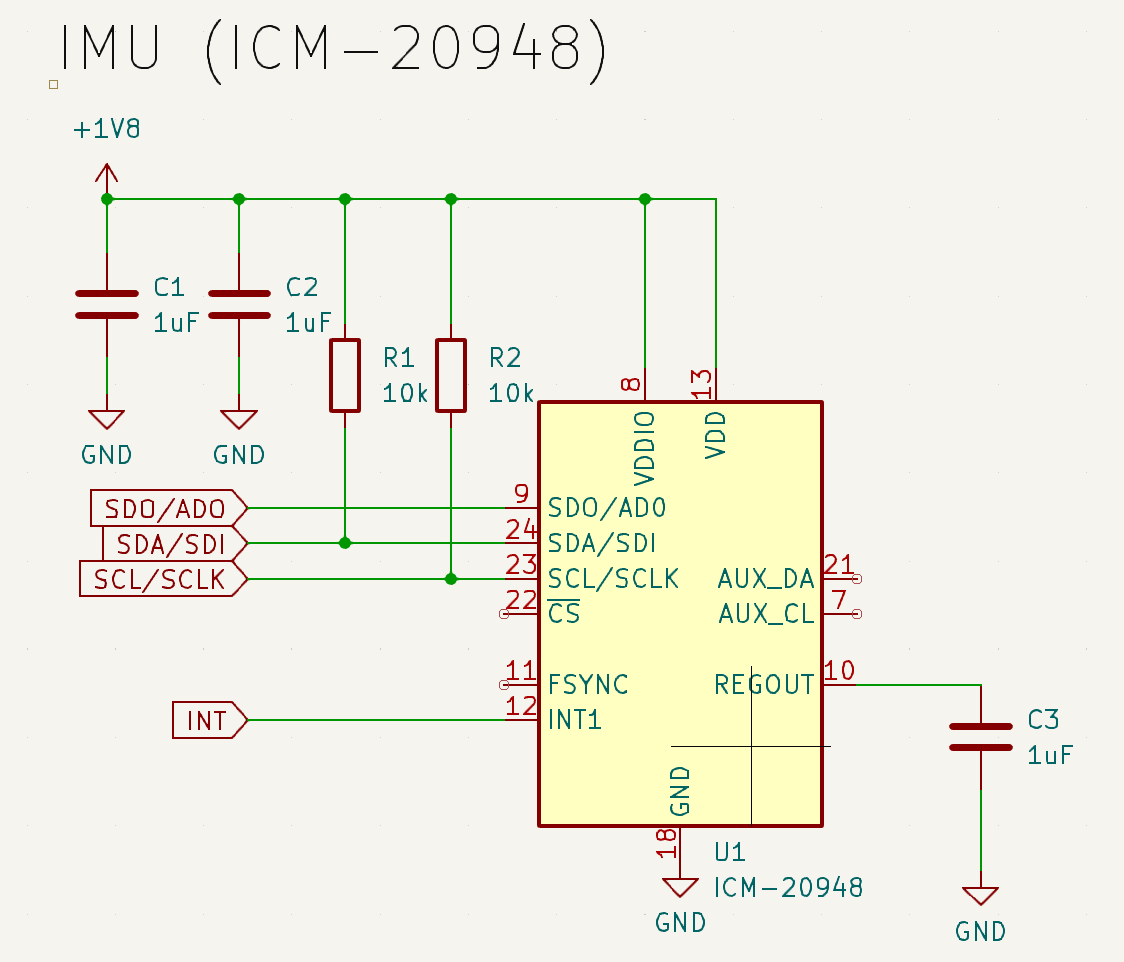
\includegraphics[width=0.8\textwidth]{images/IMU_schematic.png}
    \caption{IMU schematic}
    \label{fig:IMU_breakout}
\end{figure}
\subsubsection{Software}
It is likely that the data from the IMU will be noisy and require filtering to accurately interpret the user's gestures. The noise will cause the data from the IMU to be inaccurate after a short period of time. I am currently researching different filtering techniques to implement on the control unit to minimize noise. One possible filtering technique is the Kalman filter, which is a recursive algorithm that estimates the state of a system from a series of noisy measurements. The Kalman filter is particularly useful for systems with a high degree of uncertainty, such as the IMU data \cite{Palanisamy2016}.

I am also considering using a Recurrent Neural Network (RNN) with long short term memory (LSTM) to interpret the data from the IMUs. An RNN is a type of neural network that is well-suited for sequential data, such as the time-series data from the IMUs because it can learn the patterns in the data and make predictions based on the previous data points. The LSTM architecture is particularly useful for time-series data because it can remember information from previous time steps and use it to make predictions about future time steps \cite{IBM_RNN}. A RNN with LSTM has a connection going forward to learn from previous data.
Additionally, see figure \ref{fig:RNN} for a high-level overview of how an RNN with BiLSTM works, where there are two connections, one from the original LSTM going forward, and one going backwards to learn from future data. 

\begin{figure}[ht]
    \centering
    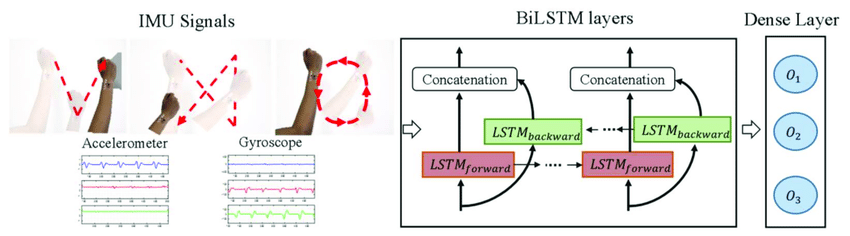
\includegraphics[width=1.0\textwidth]{images/RNN_BiLSTM.png}
    \caption{RNN with BiLSTM high level diagram \cite{ValarezoAnazco2021}}
    \label{fig:RNN}
\end{figure}

The RNN would be trained on a dataset of gestures to learn the patterns in the data and predict the user's intended gesture. This approach would require a significant amount of data to train the RNN, so it is likely we adapt an existing gesture recognition model to our specific use case. This is still in the beginning stages of research, and I will continue to explore this option as we progress in the project.
\subsection{Testing/Verification}
Testing and verification for the sensor subsystem will be done in two stages: first, testing the communication between the IMUs and the control unit, and second, testing the filtering of the IMU data. The first stage will involve sending data from the IMUs to the control unit and verifying that the data is being transmitted correctly. This will involve writing test code to read the data from the IMUs and send it to the control unit via the I2C protocol. The second stage will involve filtering the data from the IMUs to minimize noise and ensure that the control unit can accurately interpret the user's gestures. This will involve writing test code to apply different filtering techniques to the IMU data and verifying that the filtered data is more accurate than the raw data.
\subsubsection{Communication}
For the first stage, we will write test code to read the data from the IMUs and send it to the control unit via the I2C protocol. We will first be using the dev board for the ESP32 and pre made breakout boards purchased from Amazon to test the communication between the IMUs and the control unit. Once we have verified that the communication is working correctly, we will complete the custom PCB for the IMU breakout board and test the communication with the custom PCB for the control unit. The communication will be tested by sending data from the IMUs to the control unit and verifying that the data is being transmitted correctly. This will involve writing test code to read the data from the IMUs and send it to the control unit via the I2C protocol.
\subsubsection{Software}
For the second stage, we will write test code to apply different filtering techniques to the IMU data and verify that the filtered data is more accurate than the raw data. We will first test the filtering techniques on the dev board for the ESP32 and pre made breakout boards purchased from Amazon. Once we have verified that the filtering is working correctly, we will complete the custom PCB for the control unit and test the filtering with the custom PCB. The filtering will be tested by applying different filtering techniques to the IMU data and verifying that the filtered data is more accurate than the raw data.

For the RNN, we will first train the model on a dataset of gestures to learn the patterns in the data and predict the user's intended gesture. We will then test the model on a separate dataset of gestures to verify that the model can accurately interpret the user's gestures. This will involve writing test code to apply the model to the dataset of gestures and verifying that the model can accurately predict the user's intended gesture. Once the model performs well on the test dataset, we will integrate it into the control unit and test it with the IMUs to verify that it can accurately interpret the user's gestures in real-time. It is likely that we will need to optimize the model fro deployment on the microcontroller to ensure that it can run in real-time; this might involve reducing the complexity of the model via techniques such as pruning or using a more efficient implementation of the model.
\section{Conclusion}
this is the conclusion 
\newpage
\bibliography{references}


\end{document} 